\documentclass[12pt]{article}
\setlength{\oddsidemargin}{0in}
\setlength{\evensidemargin}{0in}
\setlength{\textwidth}{6.5in}
\setlength{\parindent}{0in}
\setlength{\parskip}{\baselineskip}

\usepackage{amsmath,amsfonts,amssymb}
\usepackage[english]{babel}
\usepackage{graphicx}
\usepackage{fancyhdr}
\usepackage{hyperref}
\usepackage{color}
\usepackage{amsmath}
\hypersetup{
    colorlinks=true,
    linkcolor=blue,
    filecolor=magenta,
    urlcolor=cyan,
}
\pagestyle{fancy}


\begin{document}

\lhead{{\bf Nikolai Alexander \\ Final Project} }
\rhead{{\bf December 8, 2018\\ CSCI 3104, Algorithms}}
\renewcommand{\headrulewidth}{0.4pt}


\vspace{2mm}
\noindent
\begin{enumerate}

	\item (15 pts) Doctor Jean needs your help! She's been relabeling her collection of chromosome sequences and has found three different sequences that were displaced from their original locations in the lab. She knows that two of the sequences represent two chromosomes from a human (Homo Sapiens) and the other sequence represents a chromosome from a soybean (Glycine Max).

    Help Doctor Jean by parsing in the following sequences into memory (be careful of newlines!) and applying the Longest Common Subsequence algorithm learned in recitation to each unique pair of sequences.
    
    Unzip the "sequence\_data.zip" file located on Canvas to access the data. When backtracing through the computed two dimensional matrix to find the longest common subsequence, break ties uniformly at random. Compare the results from your implementation to determine which species the sequences pertain to (try to come up with a sensible metric that will compare the results). \begin{enumerate}
    \item Show a table that maps the sequence to the species.

	{\color{blue}

		\begin{table}[h!]
		\centering
		\begin{tabular}{|l|l|}
		\hline
		\textbf{Sequence} & \textbf{Species} \\ \hline
		Sequence\_A        & Soybean          \\ \hline
		Sequence\_B        & Human            \\ \hline
		Sequence\_C        & Human            \\ \hline
		\end{tabular}
		\end{table}

		\begin{figure}[h!]
		\begin{center}
		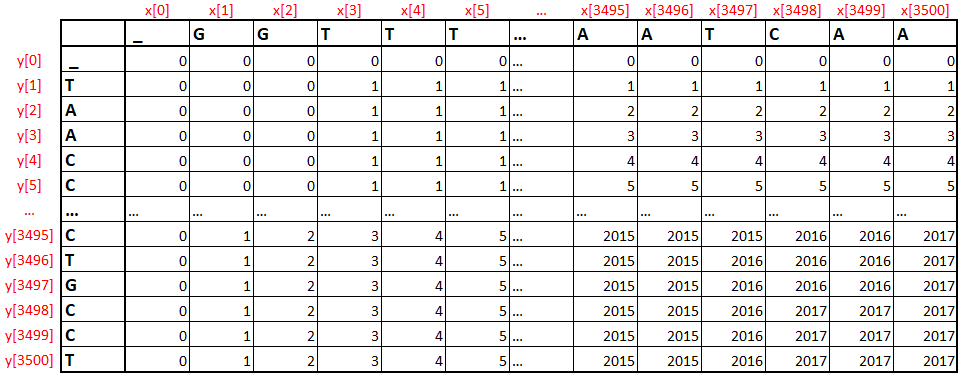
\includegraphics[scale=.6]{AB_Table.png}
		\end{center}
 		\caption{Longest Common Subsequence table comparing Sequence\_A and Sequence\_B.}
		\vspace{-4mm}
		\end{figure}

		\begin{figure}[h!]
		\begin{center}
		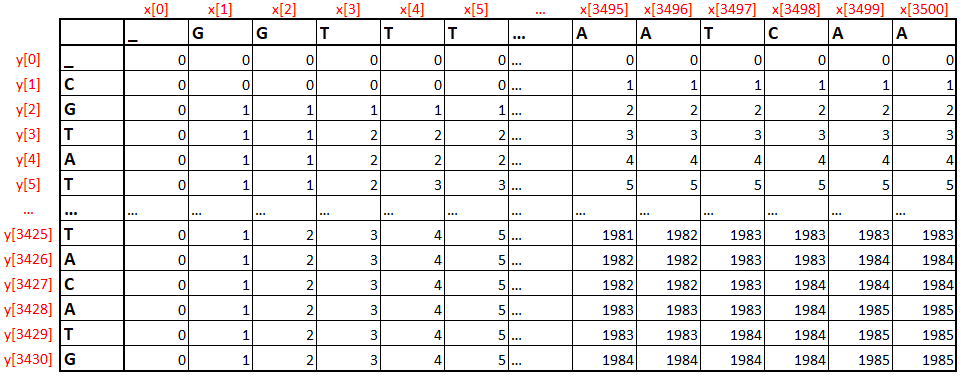
\includegraphics[scale=.6]{AC_Table.png}
		\end{center}
 		\caption{Longest Common Subsequence table comparing Sequence\_A and Sequence\_C.}
		\vspace{1cm}
		\end{figure}

		\begin{figure}[h!]
		\begin{center}
		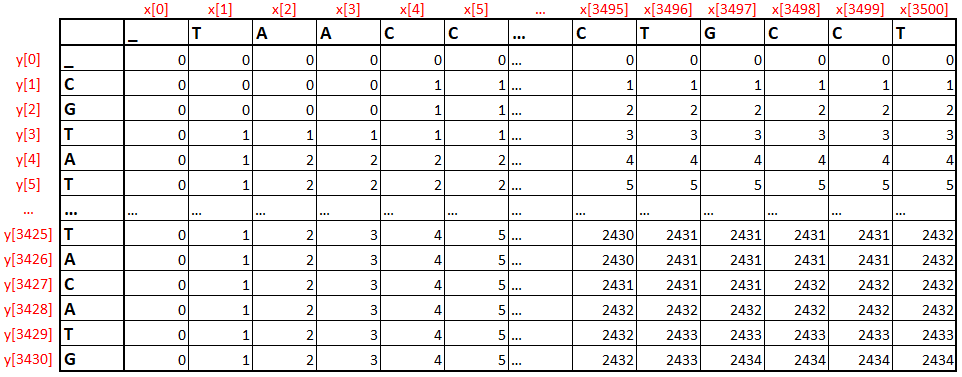
\includegraphics[scale=.6]{BC_Table.png}
		\end{center}
 		\caption{Longest Common Subsequence table comparing Sequence\_B and Sequence\_C.}
		\vspace{1mm}
		\end{figure}\newpage

		The sequences with the largest \emph{Longest Common Subsequence} are \texttt{Sequence\_B} and \texttt{Sequence\_C}. Since we know two of the three sequences are human and the third is a soybean, we can determine that \texttt{Sequence\_B} and \texttt{Sequence\_C} represent chromosomes from a human and \texttt{Sequence\_A} represents a chromosome from a soybean.


	}\newpage

    \item Submit your separate python (.py) file along with your PDF submission.

	{\color{blue}
		Python code is in \texttt{FinalProject\_Alexander.py} under \emph{Problem 1} with outputs for the \texttt{Longest Common Sequence}e tables for each comparison, the subsequences produced by each comparison, and the species that the sequences are attached to.
	}\newpage

\end{enumerate}

\item (15 pts) Draco Malfoy is struggling with the problem of making change for $n$ cents using the smallest number of coins. Malfoy has coin values of $v_{1}<v_{2}<\dots<v_{r}$ for $r$ coins types, where each coin's value $v_{i}$ is a positive integer. His goal is to obtain a set of counts $\{d_{i}\}$, one for each coin type, such that $\sum_{i=1}^{r}d_{i}=k$ and where $k$ is minimized.
	\begin{enumerate}
	\item A greedy algorithm for making change is the \textbf{wizard's algorithm}, which all young wizards learn. Malfoy writes the following pseudocode on the whiteboard to illustrate it, where $n$ is the amount of money to make change for and $v$ is a vector of the coin denominations:
	%
	\begin{small}
	\begin{verbatim}
	wizardChange(n,v,r) :
	   d[1 .. r] = 0       // initial histogram of coin types in solution
	   while n > 0 {
	      k = 1
	      while ( k < r and v[k] > n ) { k++ }
	      if k==r { return 'no solution' }
	      else { n = n - v[k] }
	   }
	   return d
	\end{verbatim}
	\end{small}
	Hermione snorts and says Malfoy's code has bugs. Identify the bugs and explain why each would cause the algorithm to fail.
	
	{\color{blue}
		There is a of number bugs I found in the code:
		\begin{enumerate}

			\item In the nested while loop, \texttt{v[k] > n} should be \texttt{v[k] <= n}. You can't make change with a coin that is of higher value than the change you need. Also, in the case that \texttt{v[0]} is less than n (which is highly likely), it would just never enter that while loop.

			\item The coditional statement for no solution \texttt{if k = r} should be \texttt{if v[0] > n} for returning no solution. We can still technically find a solution by using the largest coin. However, if we cannot reduce \texttt{n} to 0 using the smallest valued coin \texttt{v[0]}, then we cannot find a solution for exact change.

			\item Also for this same conditional statement conditional statement, \texttt{if v[0] > n} should be moved outside of the while loop. If the value of the smallest coin is greater than the value of \texttt{n}, then there is no solution, and there is no point in iterating through the larger coins in \texttt{v}.

			\item (\emph{Tenative}) Unless I'm misreading this line of pseudocode, \texttt{return 'no solution'} should be \texttt{return NULL}. \texttt{return 'no solution'} is returning a string, when we want to return no value if we cannot get the correct change. However, if this is an accepted way to write \texttt{NULL} in pseudocode, then this is not a bug.

			\item In \texttt{else} of the conditional statement, \texttt{n = n - v[k]} should be \texttt{n = n - v[k-1]}. Since we go through the nested while loop until we reach a coin larger than \texttt{n}, we need to backtrack 1 index to the largest coin that is less than \texttt{n}. We also need to make sure we call the largest element in \texttt{v} if we reach the end of the list. So, the errors this bug would bring forth are returning the wrong change completely, or giving an overrun index error.

			\item The last bug I found was also in the else part of the conditional statement: Nothing is added to \texttt{d} in the function. Therefore, we need to add \texttt{d[k-1] += 1} either right before or right after \texttt{n = n - v[k-1]}.
		\end{enumerate}

		So, with all of the bugs identified and fixed, the new algorithm should look like:
		\begin{small}
		\begin{verbatim}
			wizardChange(n,v,r) :
			     d[0:r] = 0
			     while n > 0 {
			          k = 1
			          if v[0] > n { return NULL }
			          while ( k < r and v[k] <= n ) { k++ }
			          d[k-1] += 1
			          n = n - v[k-1]
			     }
			     return d
		\end{verbatim}
		\end{small}
	}


	\item Sometimes the goblins at Gringotts Wizarding Bank run out of coins, and make change using whatever is left on hand. Identify a set of U.S. coin denominations for which the greedy algorithm does not yield an optimal solution. Justify your answer in terms of optimal substructure and the greedy-choice property. (The set should include a penny so that there is a solution for every value of $n$.)

	{\color{blue}
		A \emph{greedy algorithm} gives an optimal solution when the following properties are true:
		\begin{enumerate}
			\item \emph{Greedy Choice Property}: there is always an optimal solution that starts with greedy choice.
			\item \emph{Optimal Substructure Property}: the optimal solution to a problem contains within it optimal solutions to subproblems.
		\end{enumerate}
		Consider a set of U.S. coin denominations \texttt{v = [0.01, 0.10, 0.25, 0.50, 1.00]}. We can prove that this will not always produce and optimal solution with a proof by contradiction:

		Consider the case, where the \texttt{wizard's algorithm} is trying to return change for $\$1.80$. The first choice the greedy algorithm makes is $\$1.00$, reducing the change to $\$0.80$. Its next choice is $\$0.50$, reducing the change to $\$0.30$. After that, it chooses $\$0.25$, since that is the closest coin to $\$0.30$. Finally it iterates through the loop five more times, choosing $\$0.01$. This gives us the set:
		{\center [1.00, 0.50, 0.25, 0.01, 0.01, 0.01, 0.01, 0.01] = 8 coins\endcenter}

		However, the optimal solution is actually:
		{\center [1.00, 0.50, 0.10, 0.10, 0.10] = 5 coins\endcenter}

		This violates the \emph{Greedy Choice Property} as the greedy choice of $\$0.25$ to reduce $\$0.30$ is not the optimal choice to produce the change in the least amount of coins. This also violated the \emph{Optimal Substructure Property} as the greedy choice for $\$0.30$ is not an optimal substructure of $\$1.00$. Therefore, for coin set [0.01, 0.10, 0.25, 0.50, 1.00], the greedy algorithm does not always yield an optimal solution.
	}

	\item On the advice of computer scientists, Gringotts has announced that they will be changing all wizard coin denominations into a new set of coins denominated in powers of $c$, i.e., denominations of $c^{0}, c^{1}, \dots , c^{\ell}$ for some integers $c>1$ and $\ell\geq 1$. (This will be done by a spell that will magically transmute old coins into new coins, before your very eyes.) Prove that the wizard's algorithm will always yield an optimal solution in this case. 

	Hint: first consider the special case of $c=2$.

	{\color{blue}
		We can prove that the wizard's algorithm will always yield an optimal solution for a set of coins denominated by base-$c$ by Induction. In order so show that this algorithm works for this case, we need to show that it follow the \emph{Greedy Choice Property} and the \emph{Optimal Substructure Property}, which are again defined as follows:
		\begin{enumerate}
			\item \emph{Greedy Choice Property}: there is always an optimal solution that starts with greedy choice.
			\item \emph{Optimal Substructure Property}: the optimal solution to a problem contains within it optimal solutions to subproblems.
		\end{enumerate}\newpage

		\underline{Proof by Induction}

		\emph{Base Case: c = 2}\\
		First, we need to prove that the \emph{Optimal Substructure Property} holds true. Consider a set of coins $C = [1, 2, 4, 8, ... , 2^\ell]$ and an optimal set of coins $d[1,...,k]$ such that:
		{\center $\sum_{i = 1}^{k} d_{i} = n$, where $k$ is minimized. \endcenter}
		Now consider a subset  $d'[1,...,k']$ such that,
		{\center $\sum_{i = 1}^{k'} d'_{i} = n'$, where $k'$ is minimized, \endcenter}
		where $ d' \subseteq d$. $k' < k$, and $n' < n$. Since all values of $C$ follow the property,
		{\center $C[m] = 2\,C[m-1]$, where $m = 2^\ell$, \endcenter}
		for all values of $C$. Since all coins are factors of $2$ larger than their predecessors, an optimal substructure will hold for all optimal structures of $d$. Therefore, the \emph{Optimal Substructure Property} holds for a set of coins denominated by base-$2$

		Now, we can need to prove the \emph{Greedy Choice Property}. Consider the same set of coins $C = [1, 2, 4, 8, ... , 2^\ell]$ where $\ell \geq 1$. Suppose we choose the maximum value of $C$ such that, 
		{\center $max(c) \leq n$,\endcenter}
		and continue to choose values in this fasion until we get a set,
		{\center $\sum_{i = 1}^{k} d_{i} = n$, where $k$ is minimized. \endcenter}.
		Previously, we stated all values of $C$ follow the property:
		{\center $C[m] = 2\,C[m - 1]$, where $m \geq 1$, \endcenter}
		So, every value contained in $C$ can be broken down into combinations of smaller values contained in $C$. Since this is true, we can find the optimal solution by only picking $max(c) \leq n$, and the \emph{Greedy Choice Property} holds true.

		Since the \emph{Optimal Substructure Property} and the \emph{Greedy Choice Property} hold true for a set of coins $C = [1, 2, 4, 8, ... , 2^\ell]$, the \emph{wizard's algorithm} by definition will always yeild an optimal solution in this case.\newpage

		\emph{Induction Hypothesis:}\\
		For a set of coin denominations $C = [c^0, c^1, c^2, ... , c^\ell]$ where $c > 1$ and $\ell \geq 1$, the \emph{Optimal Substructure Property} and \emph{Greedy Choice Property} hold true for the \emph{wizard's algorithm}. Thus, the \emph{wizard's algorithm} will always yield an optimal solution.\\

		\emph{Inductive Step: $c = n + 1$}\\
		Assuming the Induction Hypothesis holds true for $n$, consider a set of coins $C = [(n+1)^0, (n+1)^1, (n+1)^2, ... , (n+1)^\ell]$ and a number $p$ for which we must find an optimal set of coins $d$ contained in $C$ such that,
		{\center $\sum_{i = 1}^{k} d_{i} = p$, where $k$ is minimized. \endcenter}
		In order to prove that the \emph{wizard's algorithm} always produces an optimal solution for set $C$, we must show that it follows the \emph{Optimal Substructure Property} and the \emph{Greedy Choice Property}.

		To show  the \emph{Optimal Substructure Property} holds true,  Consider the subset $d'$ such that,
		{\center $\sum_{i = 1}^{k'} d'_{i} = p'$, where $k'$ is minimized, \endcenter}
		where $ d' \subseteq d$. $k' < k$, and $p' < p$. The values of $C$ hold a similar pattern to that of the base case,
		{\center $C[m] = (n+1)C[m-1]$, where $m \geq 1$, \endcenter}
		This property allows us to find optimal solutions to the subproblem $p'$ since all values of $C$ are all factors of $(n+1)$ of each other. Thus, an optimal substructure will hold and the \emph{Optimal Substructure Property} always hold true for the \emph{wizard's algorithm}.

		For the \emph{Greedy Choice Property}, now consider we build a subset of C where we repeatedly choose the maximum value contained in $C$ such that
		{\center $max(c) \leq p$,\endcenter}
		until the sum of the elements in subset $d$ is equal to $p$. Because each value in $C$ is a factor $(n+1)$ apart from it's relative elements, each value in $C$ can be built from combinations of smaller elements. As a result of this property, we will always get the optimal substructure when picking the maximum value of $C$ less than $p$. Therefore, the \emph{Greedy Choice Property} holds true.

		Because the \emph{wizard's algorithm} fulfills both the \emph{Optimal Substructure Property} and the \emph{Greedy Choice Property}, it will always yield an optimal solution for any set of coin denominations of a power of c.
	}\newpage

	\end{enumerate}

	
\item In the two-player game “Pandas Peril”, an even number of cards are laid out in a row, face up. On each card, is written a positive integer. Players take turns removing a card from either end of the row and placing the card in their pile. The player whose cards add up to the highest number wins the game.
One strategy is to use a greedy approach and simply pick the card at the end that is the largest. However, this is not always optimal, as the following example shows: (The first player would win if she would first pick the 4 instead of the 5.)

4 2 10 5

\begin{enumerate}
\item (10 pts) Write a dynamic programming algorithm for a strategy to play Pandas Peril. Player 1 will use this strategy and Player 2 will use a greedy strategy of choosing the largest card.

	{\color{blue}
		\begin{small}
		\begin{verbatim}
			PandasPeril_Dynamic(A) :
			     sum1 = A[0]
			     sum2 = A.length - 1
			     choice = NULL

			     // Game 1 - if we choose the first card
			     i1 = 1
			     j1 = A.length-1
			     // Player 2's Turn
			     if A[i1] >= A[j1] {
			          i1++
			     }
			     else{
			          j1--
			     }
			     while i1 < j1 {
			          // Player 1's Turn
			          if A[i1] >= A[j1] {
			               sum1 += A[i1]
			               i1++
			          }
			          else {
			               sum1 += A[j1]
			               j1--
			          }


			          // Player 2's Turn
			          if A[i1] >= A[j1] {
			               i1++
			          }
			          else {
			               j1--
			          }
			     }

			     //Game 2 -  if we choose the last card
			     i2 = 0
			     j2 = A.length-2
			     //  Player 2's turn
			     if A[i2] >= A[j2] {
			          i2++
			     }
			     else {
			          j2--
			     }
			     // Continue the game until there are no cards left
			     while i2 < j2 {
			          // Player 1's Turn
			          if A[i2] >= A[j2] {
			               sum2 += A[i2]
			               i2++
			          }
			          else {
			               sum2 += A[j2]
			               j2--
			          }
			
			          // Player 2's Turn
			          if A[i2] >= A[j2] {
			               i2++
			          }
			          else {
			               j2--
			          }
			     }

			     // Choose card that produces highest sum
			     if sum1 >= sum2 {
			          choice = A[0]
			          delete A[0]
			          return choice
			     }
			     else {
			          choice = A[A.length-1]
			          delete A[A.length-1]
			          return choice
			     }
		\end{verbatim}
		\end{small}
	}

\item (10 pts) Prove that your strategy will do no worse than the greedy strategy for maximizing the sum of each hand.

	{\color{blue}
		\underline{Proof by Induction}

		\emph{Base Case: $n=2$}\\
		Consider a set of cards \texttt{A} of size $2$. Our dynamic strategy \texttt{PandasPeril\_Dynamic} picks 2 cards \texttt{A[0]} and \texttt{A[1]}. It then simulates two games, each starting with either \texttt{A[0]} or \texttt{A[1]} respectively. In each game, the first card is assigned to Player 1, and then Player 2 chooses a card. The two players then continue to greedily select and remove cards from \texttt{A} until there are no cards left in \texttt{A}. After both games complete, the sums of the hands for Player 1 in each game are compared. Since for a set of size $2$, the highest sum would be of the larget card in \texttt{A}, the card chosen by \texttt{PandasPeril\_Dynamic} would be,
		{\center \texttt{PandasPeril\_Dynamic = max(A[0],A[2]).} \endcenter}
		For the greedy strategy \texttt{PandasPeril\_Greedy}, the card selected is always the card with the value such that,
		{\center \texttt{PandasPeril\_Greedy = max(A[0],A[2]).} \endcenter}
		Therefore,
		{\center \texttt{PandasPeril\_Dynamic = PandasPeril\_Greedy.} \endcenter}

		\emph{Induction Hypothesis:}\\
		Given a set of cards \texttt{A} of size $n$, where $n \geq 2$ and is even, the dynamic strategy for maximizing the sum of a hand \texttt{PandasPeril\_Dynamic} produces a sum greater than or equal to the sum of a hand produced by the greedy strategy \texttt{PandasPeril\_Greedy}.\\

		\emph{Inductive Step: $n+2$}\\
		Now consider a set of cards \texttt{A} of size $n+2$.Our dynamic strategy \texttt{PandasPeril\_Dynamic} takes two cards \texttt{A[0]} and \texttt{A[n+1]} and simulates two games - one where \texttt{A[0]} is chosen first, and the other where \texttt{A[n+1]} is chosen first. In each game, Player 1 receives the first card, then Player 2 chooses the largest of the next two cards, and then each player takes turns selecting the largest card until there are no cards left in \texttt{A}. After both games have completed, the sums of each of Player 1's sets for each game are compared, and the card between \texttt{A[0]} and \texttt{A[n+1]} that produces the maximum sum is selected. This approach is continued until \texttt{A} is empty in the actual game.

		The greedy strategy \texttt{PandasPeril\_Greedy} just chooses each card such that, 
		{\center \texttt{PandasPeril\_Greedy += max(A[0],A[A.length-1])} \endcenter}
		until \texttt{A} is empty. Whereas \texttt{PandasPeril\_Dynamic} makes it's choice based off the equation
		{\center \texttt{PandasPeril\_Dynamic} \texttt{+=} $\begin{cases}
			\texttt{A[0]} \quad  iff \quad \texttt{sum1} \geq \texttt{sum2}\\
			\texttt{A[n+1]} \quad iff \quad \texttt{sum2} > \texttt{sum1}\\
		\end{cases}$
		\endcenter}
		Where,
		{\center
			\texttt{sum1} = $\texttt{A[0]} + \sum_{\texttt{i = len(A)-1}}^{0}\texttt{PandasPeril\_Greedy(A[0],A[i-1])}$\\
			\texttt{sum2} = $\quad \texttt{A[n+1]} + \sum_{\texttt{i = len(A)-1}}^{0}\texttt{PandasPeril\_Greedy(A[0],A[i-1])}$
		\endcenter}
		Thus, if \texttt{PandasPeril\_Greedy}'s choice produces the optimal sum, then,
		{\center \texttt{PandasPeril\_Dynamic = PandasPeril\_Greedy.} \endcenter}
		Otherwise,
		{\center \texttt{PandasPeril\_Dynamic > PandasPeril\_Greedy,} \endcenter}
		by definition. Therefore,  \texttt{PandasPeril\_Dynamic} produces a sum greater than or equal to the sum of a hand produced by \texttt{PandasPeril\_Greedy}, and our Induction Hypothesis holds. 
	}

\item (10 pts) Implement your strategy and the greedy strategy in Python and simulate a game, or two, of Pandas Peril. Your simulation should include a randomly generated collection of cards and show the sum of cards in each hand at the end of the game. 

	{\color{blue}
		Python code is in \texttt{FinalProject\_Alexander.py} under \emph{Problem 3: Pandas Peril} with outputs for 2 games, the randomly generated sets for each game, the set chosen by each player, the total sums of each set, and the winner of each game.
	}\newpage

\end{enumerate}

\item A common problem in computer graphics is to approximate a complex shape with a bounding box. For a set, $S$, of $n$ points in 2-dimensional space, the idea is to find the smallest rectangle, $R$. with sides parallel to the coordinate axes that contains all the points in $S$. Once $S$ is approximated by such a bounding box, computations involving $S$ can be sped up. But, the savings is wasted if considerable time is spent constructing $R$, therefore, having an efficient algorithm for constructing $R$ is crucial. 
\begin{enumerate}
\item (10 pts) Design a divide and conquer algorithm for constructing $R$ in O($\frac{3n}{2}$) comparisons.

	{\color{blue}
		\begin{small}
		\begin{verbatim}
			// For a set of points S
			Smallest_Rectangle(S) :
			     // Separate the x coordinates and y coordinates and find their
			     // minimum and maximum values in the set. Returns a set of two
			     // numbers where the the first is the minimum value and the second
			     // is the maximum value.
			     x = MinMax_Merge(S[ ,0])
			     y = MinMax_Merge(S[ ,1])

			     // Assign coordinates of rectangle corners
			     bottom_left = [x[0],y[0]]
			     bottom_right = [x[0],y[1]]
			     top_left = [x[1],y[0]]
			     top_right = [x[1],y[1]]

			     // Return a matrix of the coordinates of the four corners of the rectangle
			     R = [bottom_left, bottom_right, top_left, top_right]			
			     return R


			// Based off Merge-Sort method
			MinMax_Merge(A) :
			     if A.length > 1 {
			          p = floor(A.length/2)

			          // Divide
			          A1 = MinMax_Merge(A[0:p])
			          A2 = MinMax_Merge(A[p:A.length])

			          // Conquer
			          return MinMax_Compare(A1,A2)
			     }

			     return A

			MinMax_Compare(A1,A2) :
			     // Array to store minimum and maximum values
			     minmax_coords = [0,0]

			     if A1.length = 1 and A2.length = 1 {
			          minmax_coords[0] = min(A1[0], A2[0])
			          minmax_coords[1] = max(A1[0], A2[0])
			     }
			     else if A1.length {
			          minmax_coords[0] = min(A1[0], A2[0])
			          minmax_coords[1] = max(A1[0], A2[1])
			     }
			     else if A2.length {
			          minmax_coords[0] = min(A1[0], A2[0])
			          minmax_coords[1] = max(A1[1], A2[0])
			     }
			     else {
			          minmax_coords[0] = min(A1[0], A2[0])
			          minmax_coords[1] = max(A1[1], A2[1])
			     }

			     return minmax_coords
		\end{verbatim}
		\end{small}

		This algorithm works similarly to Merge-Sort, however, instead of sorting an array, it is recursively comparing the minimum and maximum values of the list. It works by dividing the array by halves until there is only 1 element left in each array. It then begins comparing the minimum and maximum elements with the respective minimum and maximum elements from the array it previously split from. For the first comparison, makes 1 comparison for each of the elements, and stores the minimum of the two in the first element of an array of size $2$, and stores the maximum of the two in the second element of the min-max array. It then returns the min-max array. The algorithm then works it's way back up the tree, recursively comparing the minimum values from two sets, and the maximum values from both sets respectively, and keeps the minimum and maximum values of those two set of comparisons. Since, the minimum values are only being compared with other minimum values and maximum values are only being compared with other maximum values, the total possible number of comparisons is $\frac{3n}{2}$
	}

\item (10 pts) Implement your algorithm in Python. Generate 50 points randomly and show that your bounding box algorithm correctly bounds all points generated. Your code should output the list of points, as well as the coordinates of $R$. You should include an explanation of the results in your pdf file with your algorithm.
\end{enumerate}

	{\color{blue}
		Python code is in \texttt{FinalProject\_Alexander.py} under \emph{Problem 4: Smallest Bounding Rectangle} with outputs for the set \texttt{S} of $50$ points with coordinates x and y, and the coordinates of the smallest rectangle containing those points \texttt{R}.

		Since the edges of the rectangle must be parallel to their respective coordinates, the dimensions of the rectangle are limited to the minimum and maximum x and y values in the set. Therefore, the y-coordinate of the top horizontal edge goes through the coordinate(s) with the maximum y-value while the bottom horizontal edge goes through the point with the minimum y-coordinate. The same applies to the horizontal edges.
	}\newpage
    
\item (10 pts) Professor Voldemort has designed an algorithm that can take any graph $G$ with $n$ vertices and determine in $O(n^k)$ time whether $G$ contains a clique of size $k$. Has the Professor just shown that $P = NP$? Why or why not?

	{\color{blue}
		Voldemort has \textbf{not} shown us that $P = NP$. A \emph{non-deterministic polynomial algorithm} ($NP$) is a decision algorithm that produces a Boolean solution, in polynomial time, as to whether a solution to a problem can be found. However, a \emph{polynomial algorithm} ($P$) is a search algorithm that produces an actual solution to a problem in polynomial time. 

Though Voldemort's NP algorithm is able to check to see if graph $G$ contains a clique of size $k$, it does nothing to prove that the clique was actually found through a search algorithm in polynomial time. Additionally, as of right now there is no proof to show that $P$ is theoretically equivalent to $NP$ in all cases. Therefore, Voldemort's NP algorithm is not enough to demonstrate that the clique of size $k$ was also found in polynomial time $O(n^k)$.
	}\newpage

\item (10 points) Consider the special case of TSP where the vertices correspond to points in the plane, with the cost defined for an edge for every pair (p, q) being the usual Euclidean distance between p and q. Prove that an optimal tour will not have any pair of crossing edges.

	{\color{blue}
		The \emph{Traveling Salesman Problem} looks for an optimal path that crosses every point and returns back to the source point with the smallest possible weight. In order to prove that an optimal tour does not have any pair of crossing paths, we need to prove that the sum of the crossing paths are longer than the sum of any two outer paths. Now, in general, TSP does not require weights between two vertices to be symmetric in both directions ($W_{(p,q)} \neq W_{(q,p)}$), or for the weights to satisfy the \emph{Triangle Inequality Theorem}. However, because in this case, the weights of the edges are the Euclidean distances between two points, this becomes a geometric problem and must satisfy both the above properties. We are going to use the \emph{Triangle Inequality Theorem} to prove our hypothesis. For simplicity, consider the below quadrilateral:

		\begin{figure}[h!]
		\begin{center}
		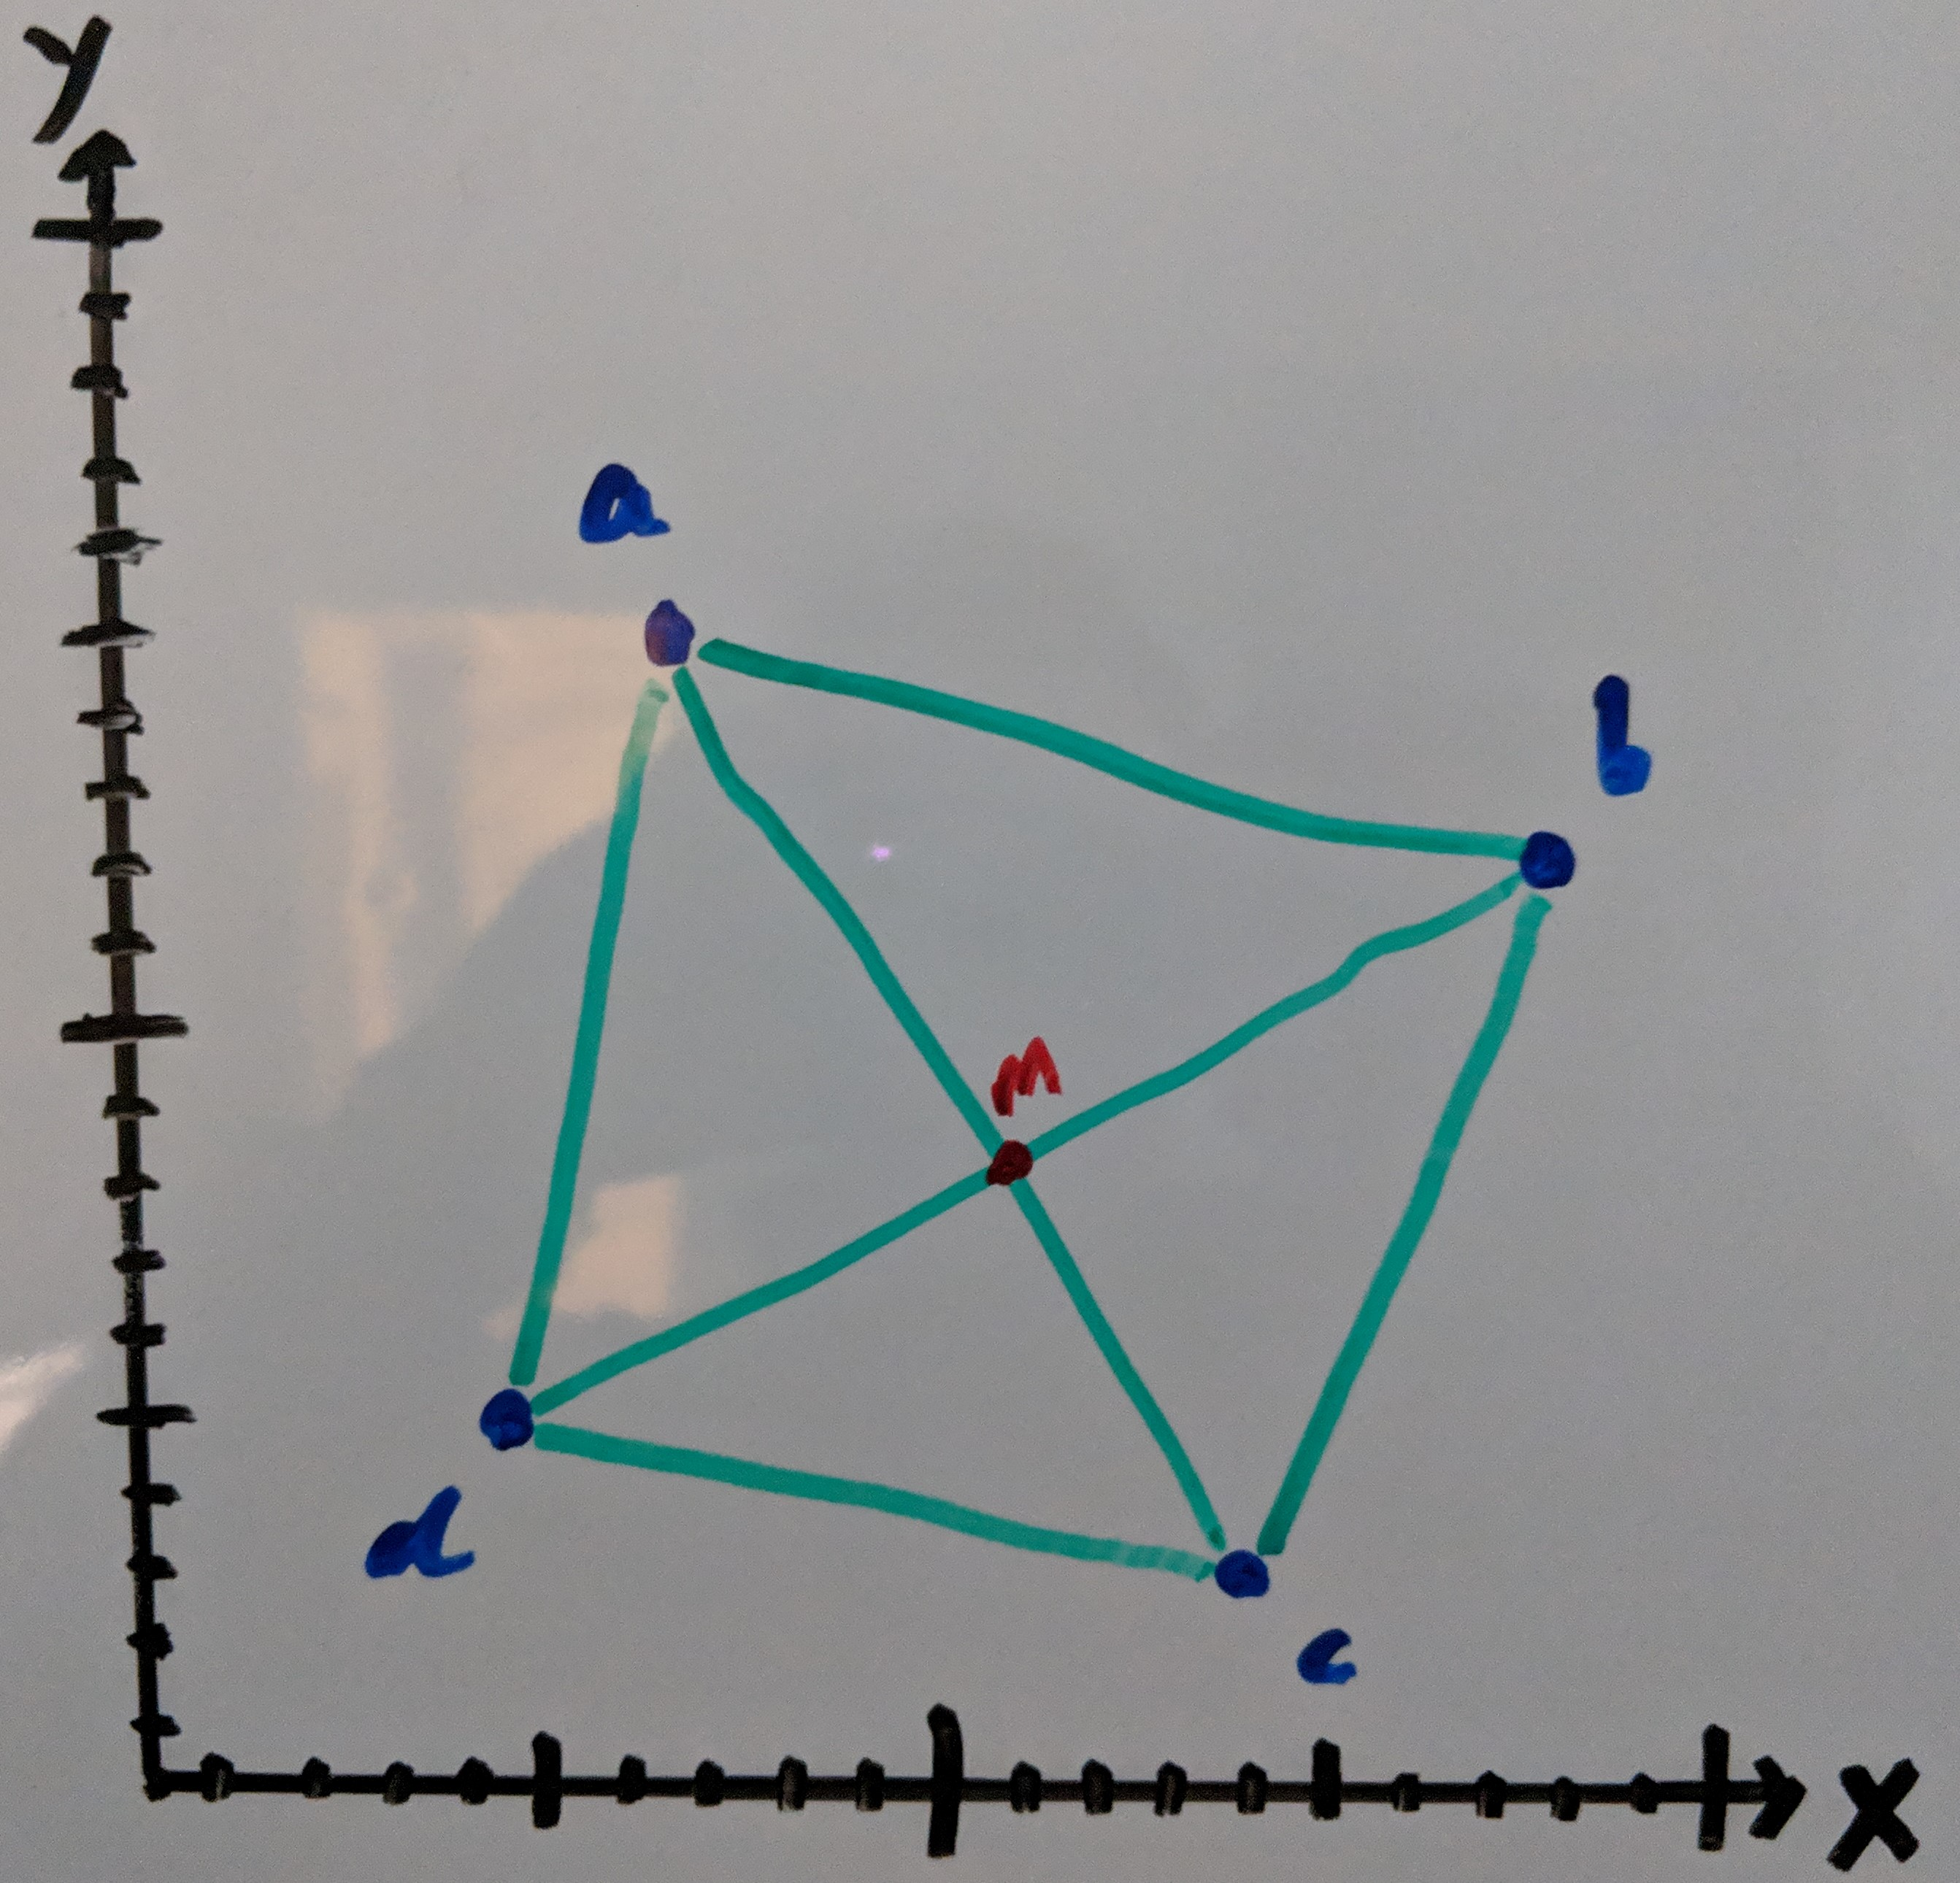
\includegraphics[scale=.1]{TSP_Quad.jpg}
		\end{center}
		\vspace{-4mm}
		\end{figure}\newpage

		For this quadrilateral , we need to find the optimal path through all four points. In order to use the \emph{Triangle Inequality Theorem}, we can place a theoretical point $m$ where (a,c) and (b,d) cross. There are three possible undirected paths we can take:
		{\center $[(a,b), (b,c), (c,d), (d,a)]$,\endcenter}
		{\center $[(a,b), (b,d), (d,c), (c,a)]$,\endcenter}
		{\center $[(a,d), (d,b), (b,c), (c,a)]$.\endcenter}
		We need to show that:
		{\center $sum(W_{(a,b)}, W_{(b,c)},W_{(c,d)}, W_{(d,a)}) < sum(W_{(a,b)}, W_{(b,d)},W_{(d,c)}, W_{(c,a)})$,\endcenter}
		{\center $sum(W_{(a,b)}, W_{(b,c)},W_{(c,d)}, W_{(d,a)}) < sum(W_{(a,d)}, W_{(d,b)},W_{(b,c)}, W_{(c,a)})$,\endcenter}
		where $W_{(p,q)}$ is the distance between points $p$ and $q$. So, the \emph{Triangle Inequality Theorem} states for a triangle $\bigtriangleup ABC$,
		{\center $W_{AB} + W_{AC} < W_{BC}$,\endcenter}
		{\center $W_{AB} + W_{BC} < W_{AC}$,\endcenter}
		{\center and $W_{AC} + W_{BC} < W_{AB}$.\endcenter}
		Now, we can use this to prove, $sum(W_{(a,b)}, W_{(b,c)},W_{(c,d)}, W_{(d,a)}) < sum(W_{(a,b)}, W_{(b,d)},W_{(d,c)}, W_{(c,a)})$. Using point $m$, where (a,c) and (b,d) cross, we can see that,
		{\center $W_{(a,m)} + W_{(c,m)} = W_{(a,c)}$,\endcenter}
		{\center and $W_{(b,m)} + W_{(d,m)} = W_{(b,d)}$.\endcenter}
		Also, since edges (a,b) and (c,d) are in both paths, we only need to show,
		{\center $W_{(b,c)} + W_{(d,a)} < W_{(b,d)} + W_{(c,a)}$.\endcenter}
		So, we can see that,\\
		$W_{(b,c)} < W_{(b,m)} + W_{(c,m)}$ for triangle $\bigtriangleup cbm$ and,\\
		$W_{(a,d)} < W_{(a,m)} + W_{(d,m)}$ for triangle $\bigtriangleup adm$.\\
		Adding these two relations we get,
		{\center $W_{(b,c)} +  W_{(a,d)} < W_{(b,m)} + W_{(c,m)} + W_{(a,m)} + W_{(d,m)}$\endcenter}
		{\center $W_{(b,c)} +  W_{(a,d)} < (W_{(a,m)} + W_{(c,m)}) + (W_{(b,m)} + W_{(d,m)})$\endcenter}
		{\center $W_{(b,c)} +  W_{(a,d)} < W_{(a,c)} + W_{(b,d)} $\endcenter}
		Thus, 
		{\center $sum(W_{(a,b)}, W_{(b,c)},W_{(c,d)}, W_{(d,a)}) < sum(W_{(a,b)}, W_{(b,d)},W_{(d,c)}, W_{(c,a)})$\endcenter}
		holds true. Now we can do the same for the other relation. Since edges (b,c) and (a,d) are in both paths, we need to show,
		{\center $W_{(a,b)} + W_{(c,d)} < W_{(b,d)} + W_{(c,a)}$.\endcenter}
		So, we can see that,\\
		$W_{(a,b)} < W_{(a,m)} + W_{(b,m)}$ for triangle $\bigtriangleup abm$ and,\\
		$W_{(c,d)} < W_{(c,m)} + W_{(d,m)}$ for triangle $\bigtriangleup cdm$.\\
		Adding these relations together,
		{\center $W_{(a,b)} +  W_{(c,d)} < W_{(a,m)} + W_{(b,m)} + W_{(c,m)} + W_{(d,m)}$\endcenter}
		{\center $W_{(a,b)} +  W_{(c,d)} < (W_{(a,m)} + W_{(c,m)}) + (W_{(b,m)} + W_{(d,m)})$\endcenter}
		{\center $W_{(a,b)} +  W_{(c,d)} < W_{(a,c)} + W_{(b,d)} $\endcenter}
		Therefore, both our above hypotheses hold true, and we have proved that an optimal tour will not have any pair of crossing edges in a TSP where the weights of the edges are the Euclidean distance between two points.

	}

\end{enumerate}
\end{document}
